\documentclass[letterpaper, 10pt, conference]{ieeeconf}

\overrideIEEEmargins

\usepackage[dvips]{graphicx}
\DeclareGraphicsExtensions{.eps}

\setlength{\parskip}{0.05cm}

% *** MATH PACKAGES ***
\usepackage[cmex10]{amsmath}
\usepackage{amssymb}
\interdisplaylinepenalty=2500

\usepackage{color}

\hyphenation{op-tical net-works semi-conduc-tor}

\newcommand\numberthis{\stepcounter{equation}\tag{\theequation}}
\newcommand{\m}[1]{\mathbf{#1}^m}

\begin{document}
\title{Is the direction of Granger causal influence the same as the direction of information flow?}
\author{Praveen Venkatesh and Pulkit Grover\\Carnegie Mellon University}

\maketitle

% Abstract --------------------------------------------------------------------

\begin{abstract}
	Granger causality is an established measure of the ``causal influence'' that one stochastic process has on another. Along with its more recent generalization -- Directed Information -- Granger Causality has been used extensively in neuroscience, and in complex interconnected systems in general, to infer causal influences. Of late, many works have begun to interpret the direction of causal influence as the direction of ``information flow''. We ask: is the direction of causal influence, as predicted by Granger Causality and Directed Information always the same as the direction of information flow? We test whether these measures correctly predict the direction of information flow by using two simple theoretical experiments, in which the true direction of information flow (the ``ground truth'') is known by design. The experiments are based on a communication system with a feedback channel, upon which a strategy inspired by the work of Schalkwijk and Kailath is employed. We show that in these experiments, the direction of information flow can be opposite to that which is inferred using Granger causality and Directed Information. Thus, while it might be reasonable to infer the direction of causal influence using these techniques, one needs to exercise care in interpreting the direction of causal influence as the direction of information flow.
\end{abstract}

\IEEEpeerreviewmaketitle

% Introduction ----------------------------------------------------------------

\section{Introduction}
\label{sec:intro}

% Intro: Motivation -----------------------------------------------------------

\subsection{Motivation}
\label{sec:motivation}

This work is in large part motivated by a recent surge of interest in understanding neural circuits -- the connectivity and dynamic activity of different regions of the brain -- and how they give rise to behavior and experience. This is evidenced by the launching of the BRAIN initiative in the US and the Human Brain Project in Europe. To quote from \emph{BRAIN 2025: A Scientific Vision}\footnote{The BRAIN Working Group's report to the Advisory Committee to the Director of the NIH}, we wish to ``map connected neurons in local circuits and distributed brain systems, enabling an understanding of the relationship between neuronal structure and function'', clearly indicating the move towards understanding (a) the connectivity and (b) the computational function of different brain regions. While the question of how the brain computes has been of immense interest for several decades, only recently have measurement techniques become sophisticated enough to be able to simultaneously record the activity of multiple neurons, or multiple neural populations.

In order to understand how the brain performs computations, it could be useful to first understand the directions of \emph{information flow} in various parts of the brain (e.g.~\cite{blinowska2004granger,dhamala2008analyzing,nolte2008robustly,korzeniewska2003determination,schippers2010mapping} etc.). In an effort to make headway on the goals of \emph{BRAIN 2025}, several works use Granger causality (and less often, its information-theoretic generalization -- Directed Information) to understand how this information flows (eg.~\cite{Brovelli2004BetaOscillations,goebel2003investigating,deshpande2008effective}), or to acquire directed maps of functional connectivity (eg.~\cite{friston2013analysing,goebel2003investigating,deshpande2008effective}). For instance, in~\cite{Brovelli2004BetaOscillations}, Granger causal influences that are measured between somatosensory and motor sites are said to ``support the idea that somatosensory feedback provides information to the sensorimotor system that is used to control motor output''. This raises the question: do these directed connectivity maps, as determined by directional causal influence measures such as Granger causality, correctly identify the directions along which information flows in the brain?

\begin{figure}[htbp] %  figure placement: here, top, bottom, or page
	\centering
	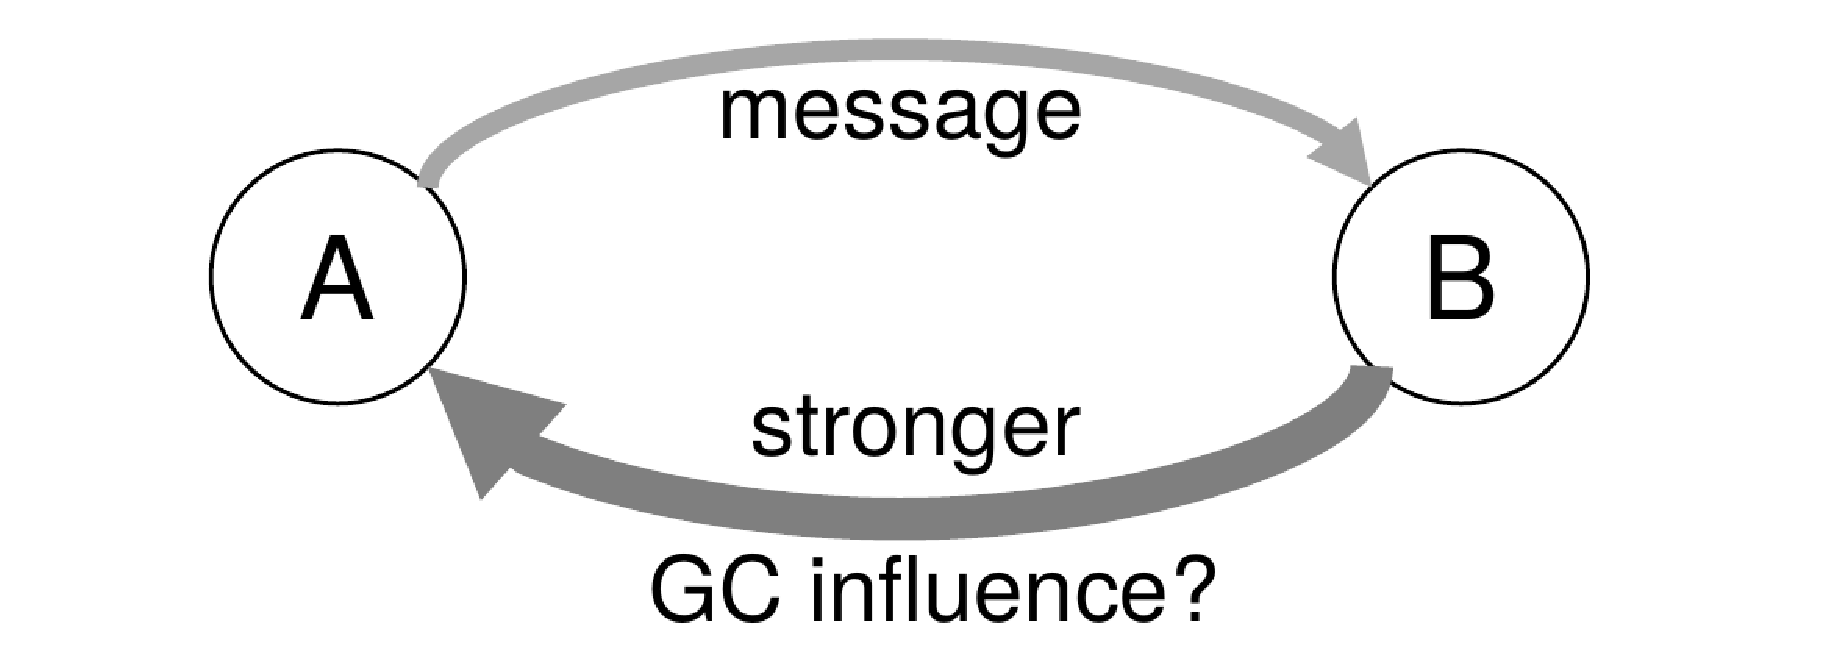
\includegraphics[width=3.2in]{gc-vs-message}
	\caption{Is the direction of stronger Granger-causal influence necessarily the same as the direction in which the information (or equivalently, the ``message'') is flowing?}
	\label{fig:gc-vs-message}
\end{figure}

% Intro: How GC is used in neuroscience today ---------------------------------

\subsection{How Granger Causality is used in Neuroscience today}
\label{sec:gc-used-in-neuroscience}

Several works have outlined the procedures involved in using Granger Causality to estimate causal influences in the brain (\cite{bernasconi2000bidirectional,Brovelli2004BetaOscillations,Ding2000ShortWindow,Roebroeck2005MappingDirected,Bressler2011WienerGranger,Barnett2014MVGC,Ding2006GrangerCausality}). Here, we briefly describe how Granger Causal influence is quantified, and how it is computed in these works.

Granger causality, as originally described by Granger~\cite{Granger1969InvestigatingCausal}, measures the level of influence that one process $\{X\}$ has on another process $\{Y\}$. The analysis compares the \emph{error in predicting} the $\{Y\}$ process based on (i) simply the past of $\{Y\}$, and (ii) based on the past of both $\{X\}$ and $\{Y\}$. The Granger causality metric is the ratio of these errors, encapsulating the innovations that the process $\{X\}$ causally supplies to the process $\{Y\}$. Many variants of Granger causality have also been considered, including a generalization -- Directed Information (see~\cite{MasseyCausality,quinn,weissman}) -- an information-theoretic quantity denoted by $I(\m{X}\to\m{Y})$. These variants form possible alternatives for estimating the direction of causal influence, but Directed Information is a generalization of many of these metrics~\cite{quinn}.

The computation of Granger causality, in general, requires that the processes under consideration be stationary. In neuroscientific experiments, this is usually not the case, as the express objective of the experiment is to understand brain function while the brain is subjected to a task. Typically, data analysis techniques either assume stationarity regardless, or circumvent the problem by working with time-windows short enough that the processes \emph{are} in fact stationary within those windows~\cite{Ding2000ShortWindow}. In the latter case, Granger causal influences are computed for each window individually, in order to produce a dynamic description of brain connectivity as the brain carries out the said task. The Granger Causality metrics can be accurately computed even for short time windows, because neuroscientific experiments usually have multiple trials, i.e.\ multiple realizations of the same processes, allowing for fitting regression coefficients accurately~\cite{Ding2000ShortWindow}.

\begin{figure}[htbp] %  figure placement: here, top, bottom, or page
	\centering
	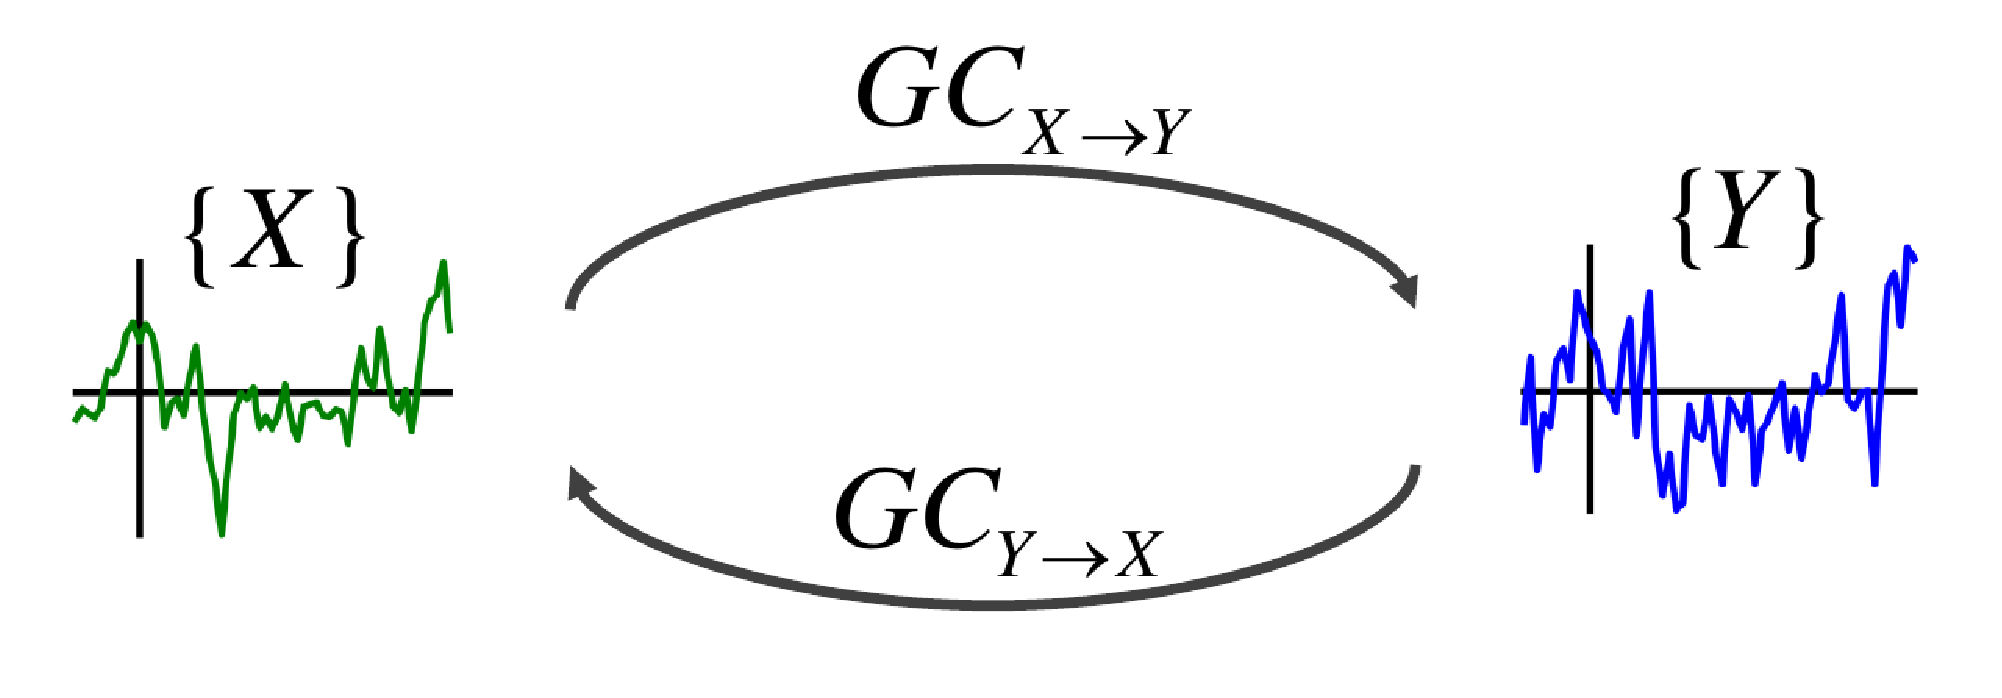
\includegraphics[width=3.2in]{gc-comparison}
	\caption{In order to determine the direction of greater causal influence, the Granger Causality metrics in the forward and reverse directions are compared}
	\label{fig:gc-comparison}
\end{figure}

In order to determine the direction of greater causal influence, the Granger Causality metric (ratio of residual variances) from $\{X\}$ to $\{Y\}$ is \emph{compared} to that from $\{Y\}$ to $\{X\}$. The direction of causal influence is taken to be the direction with a greater Granger Causality metric. Further, this direction of causal influence is interpreted to be the direction of information flow -- the interpretation we question in this paper. We also note that many of these works use a spectral version of Granger Causality, that supplies this metric as a function of frequency. It then becomes possible to also determine the brain wave frequency at which these influences occur. However, we restrict our analysis to the simpler non-spectral version of Granger Causality, since it is sufficient to for the purpose of our arguments.

We note here that Granger's original analysis does not compare this metric on forward and reverse links, however, this is commonly done in practice even in areas beyond neuroscience (eg.~\cite{Brovelli2004BetaOscillations,jiao2013universal}).

While we accept that Granger Causal influence can be accurately computed (provided measurements are taken suitably; see Section~\ref{sec:previous-criticisms-of-gc}) and can be useful in many situations (see Section~\ref{sec:conclusions}), interpreting the direction of Granger Causal influence as the direction of information flow can be erroneous, as we demonstrate in this paper.

% Intro: Previous criticisms of GC --------------------------------------------

\subsection{A short survey of previous criticisms of Granger Causality}
\label{sec:previous-criticisms-of-gc}

Several objections have been leveled against Granger Causality in the past. We give, here, a short overview of these and describe why our objection is novel, and possibly more fundamental in nature, at least in the context of its usage in neuroscience.

\begin{enumerate}
	\item First, Granger Causality suffers from what we call the ``hidden node problem''. If two observed nodes receive causal influences from a third, latent node, then a causal influence may be detected between the observed nodes, even if they are independent of each other~\cite{pearl2009causality-hidden-node}. All nodes need to be observed, therefore, to avoid finding spurious influences.
	\item Second, if the measurements from each node are differentially affected by noise, then the predicted direction of causal influence might be opposite to the true direction (\cite{nalatore2007mitigating,andersson2005testing}). Measurements need to be relatively noiseless and precise in order to obtain the correct direction of causal influence.
	\item Third, subsampling the processes can produce misleading Granger Causal relations~\cite{gong2015discovering}. Performing Granger Causal analysis on subsampled time series can lead one to miss the causal influence. If pre-processing involves subsampling, then this should be done with care.
\end{enumerate}

It is important to note that the technical objections listed above are all deficiencies in or limitations of \emph{measurement}. They indicate that incorrect Granger Causal influences may be computed if there is some deficiency or limitation in the measurement procedure. These objections can be resolved by taking better measurements (by sampling more nodes, with higher signal-to-noise ratio, etc.).

Our objection, on the other hand, is more fundamental. \emph{Even if} the measurements are made with infinite accuracy, and the regression coefficients associated with computing Granger Causality are precisely estimated, and the Granger Causality metric is perfectly computed (as is the case in our counter-examples), Granger Causal influence may \emph{still} not yield the correct direction of information flow. To our knowledge, the argument that Granger causal influence can be opposite to the direction of information flow is a novel one. We believe that this argument is much more serious than previous objections, at least in the context of determining the directions of information flow in neuroscientific experiments, towards understanding the computational functions of brain regions.

% Intro: Our counter-examples -------------------------------------------------

\subsection{Our counter-examples and our main result}
\label{sec:our-counterexamples}

This paper considers two experiments (introduced in Section~\ref{sec:sk}) where a transmitter $Tx$ wants to communicate a message to a receiver $Rx$ in presence of a feedback channel (in one experiment, the feedback link is noiseless, while in the other it is noisy). We assume that the experimenter is able to record the transmissions of $Tx$ and $Rx$ using some probing mechanism. Provided with these measurements, the experimenter wants to estimate the direction of information flow, which in this context is the direction of flow of the message. Our results, derived in Section~\ref{sec:analytical-results} and numerically illustrated in Section~\ref{sec:numerical-results}, show that both Granger causality and Directed Information can incorrectly estimate the direction of information flow. The first experiment considers the (unrealistic) case of communication across noiseless feedback channels. The second experiment allows for noise in the feedback channel. In both cases, linear strategies inspired from the scheme of Schalkwijk and Kailath~\cite{S&K} are used.

Our goal here is to bring out the point that whether Granger causality and Directed Information can be used to interpret direction of information flows is an issue that can be, and perhaps should be, considered using thought experiments on simple communication problems where \emph{information flow direction, and quantity, is already known}. If the direction of causal influence yielded by Granger causality or some other similar measure were to match the known direction of information flow, then that measure can be more confidently used in experiments. While our results strongly suggest that one needs to exercise care in interpreting Granger causality and Directed Information dominance as an indicator for the direction of information flow, there are several shortcomings that need to be addressed in order to understand the issue at depth. These shortcomings are discussed in detail in Section~\ref{sec:objections-and-shortcomings}.

We find it interesting to note that the mathematical machinery used in this paper amounts to routine arithmetic. Even simple counter-examples that do not employ difficult proof techniques are able to demonstrate our main result. This simplicity leads us to think that this counter-example is not very special, and that directions of stronger Granger Causal influence and information flow might have little to do with each other in more complex and/or noisy networks.

% Intro: Possible objections and shortcomings ---------------------------------

\subsection{Possible objections to, and shortcomings of this work}
\label{sec:objections-and-shortcomings}

A review of a submission to a previous conference raised some objections to this work, which we discuss to clarify our perspective. Further, our analysis has certain shortcomings, which we acknowledge. These will form the basis for future work.

\begin{enumerate}
	\item Firstly, and most importantly, previous work has already shown that presence of a Granger Causal influence does not imply true causation. Judea Pearl classifies Granger Causality as stemming from a ``statistical'' model, rather than from a ``causal'' model~\cite{pearl2009causality-gc-stat}. A potential issue, therefore, might be the question the novelty of this work, given that Pearl's classification could be seen to clear up the misconception. While our argument is, in spirit, very similar to this criticism of Granger causality, in the situation we study, we ask a different question - we wish to understand whether or not Granger Causality gives the correct direction of \emph{information flow}. Further, we give a concrete counter-example in this context, which is very relevant in the modern neuroscience setting.
	\item Our analysis does not tackle an information source that evolves with time. Hence, our communication process (inspired from the scheme of Schalkwijk and Kailath~\cite{S&K}) is non-ergodic. Since Granger causality is really just relative errors in prediction of a process, in presence or absence of knowledge of another process, we compute the obvious generalization of Granger causality to non-ergodic processes. Nevertheless, future work will address a situation with a linear dynamical system as the information source.
	\item Our experiments restrict themselves to Gaussian noise for simplicity, but neural spiking and spike-rate models for spikes tend to be very different from those used here. This is a clear direction for future work.
	\item The power and energy constraints are somewhat oversimplified to make the analysis simpler. This is for simplicity of exposition. A more general analysis is a trivial extension.
	\item We have also restricted ourselves to analyzing linear feedback communication strategies. In the presence of noise in the feedback link, linear communication strategies are known to be sub-optimal~\cite{YoungHanKimPaper}. In order to make a water-tight argument, we would need to show that Granger Causality fails to correctly predict the direction of information flow, even when an optimal communication strategy -- which would have to be non-linear. This could be scope for future work. However, we do not expect results to change dramatically -- when the feedback link is impaired by noise of only very low variance, the noiseless case should make for a good approximation of the system, and results should degrade gracefully, if there is any degradation at all.
	\item We consider a simple point-to-point network. In general networks, this issue could be even more complex. However, since this issue shows up even for the simplest network, we feel that the problem will only be exacerbated when the network is large.
\end{enumerate}

%Notes:
%You only seem to be assuming that the variance is $\sigma_\theta^2$. Nothing about whether it is a uniform random variable or something derived from quantizing a uniform random variable, or a Gaussian one.

% Schalkwijk and Kailath scheme description -----------------------------------

\section{A simple feedback communication scheme}
\label{sec:sk}

\begin{figure}[htbp] %  figure placement: here, top, bottom, or page
	\centering
	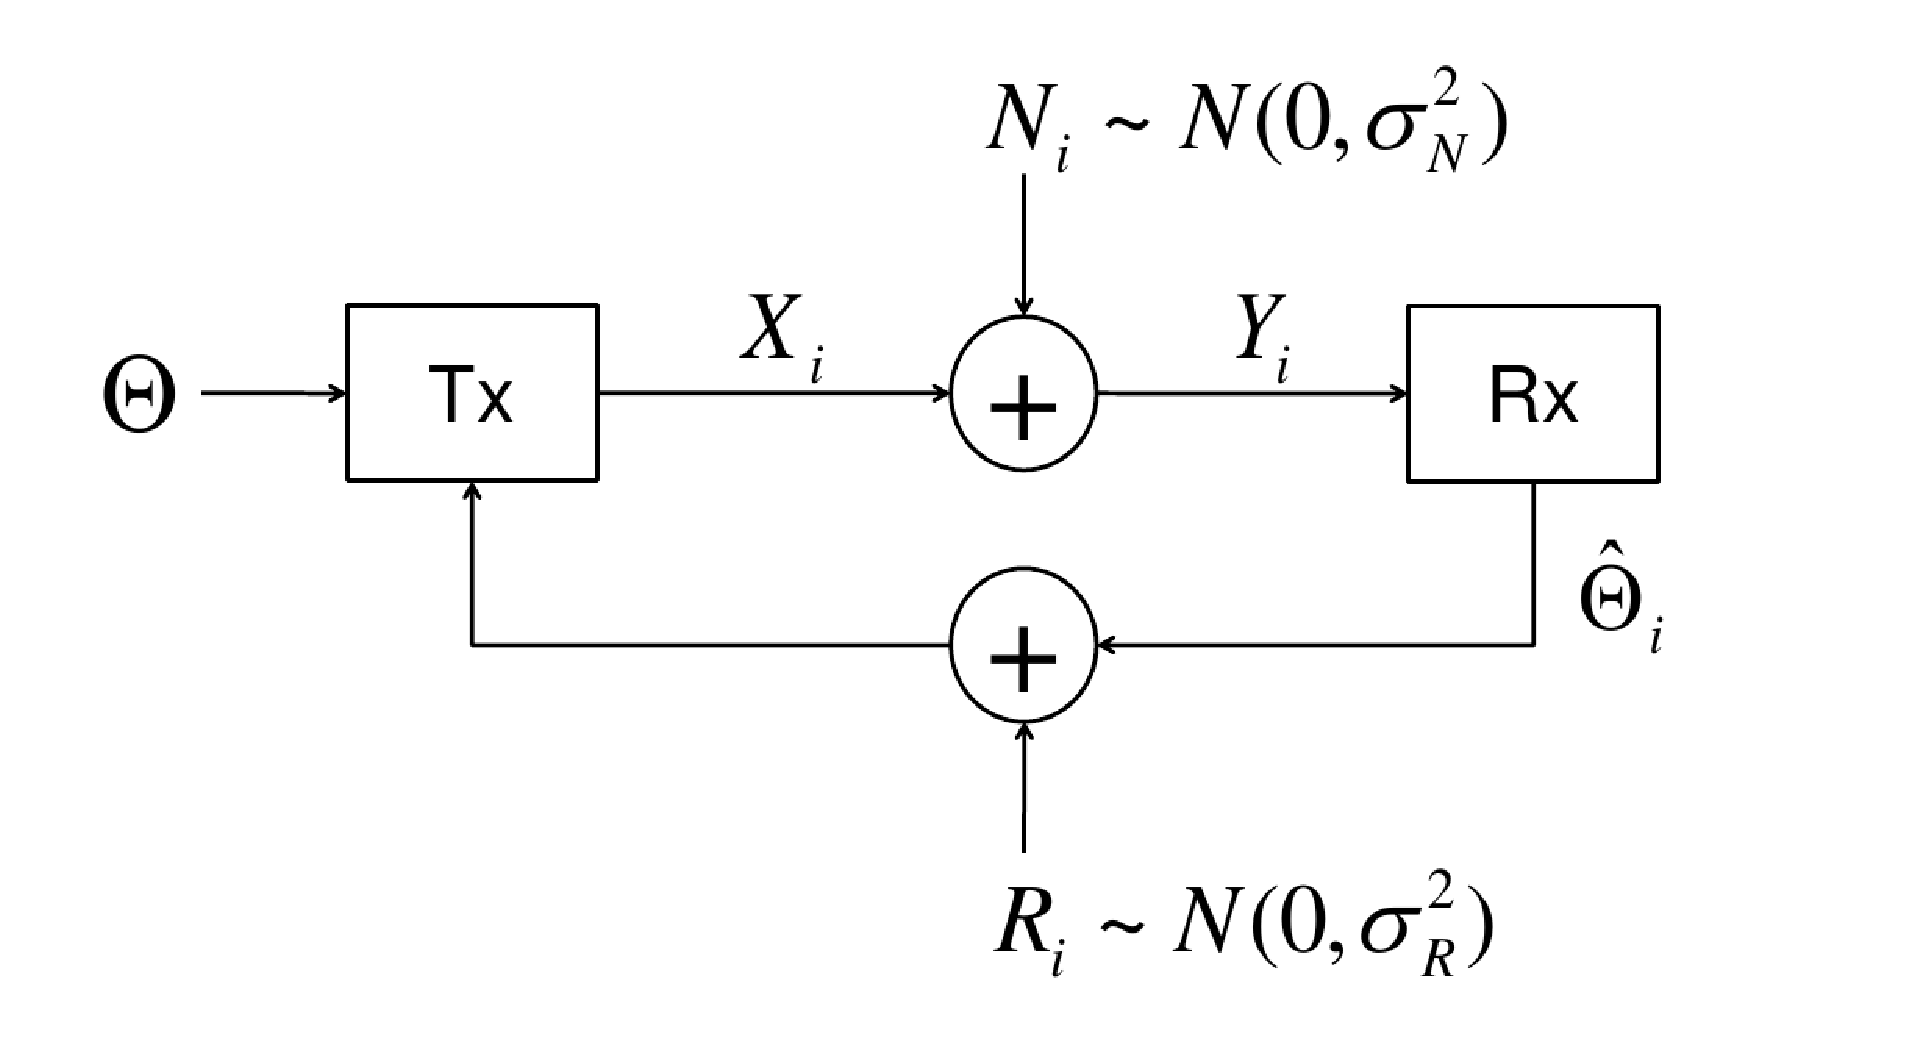
\includegraphics[width=3.2in]{sk-block-diagram}
	\caption{A block-diagram representation of the communication system, describing the feedback channels and supplying notation for the variables used throughout the paper. Note that this diagram is the more general of the two cases discussed in sub-sections~\ref{sec:sk-noiseless} and~\ref{sec:sk-noisy}, as it contains noise in the feedback link. The former, noiseless, case is equivalent to setting $\sigma_R^2$ to 0.}
	\label{fig:sk-block-diagram}
\end{figure}

This section summarizes the analysis in the work of Schalkwijk and Kailath~\cite{S&K}, and a simple (and previously known) extension to a noisy feedback case. It also establishes the model and the notation used in the paper.

The transmitter wants to convey a single zero-mean random number, $\Theta$, having variance
$\sigma_\theta^2$, to the receiver. $\Theta$ could be obtained, for instance, by quantizing a bounded interval on the real line (e.g. $[-1,1]$), as is done in the scheme of Schalkwijk and Kailath~\cite{S&K}. The forward channel is an AWGN channel with noise variance $\sigma_N^2$. We will use simple linear communication strategies for a noiseless feedback channel, as well as an AWGN feedback channel with noise variance $\sigma_R^2$. In both cases, the estimators will be shown to be unbiased and consistent (the error mean is zero, and the error variance converges to zero).

% S&K: Noiseless feedback -----------------------------------------------------

\subsection{Noiseless feedback: the Schalkwijk-Kailath strategy}
\label{sec:sk-noiseless}

 In the first step, the transmitter sends\footnote{We assume that the power constraints are such that the scaling constant $\alpha$ in~\cite{S&K} is $1$.} $X_1 = \Theta$, which the receiver receives with added noise. The receiver sends back an estimate of $\Theta$ over the feedback link. In all subsequent iterations, the transmitter sends the receiver the error in its latest estimate.

Therefore, in general, the transmitter sends
\begin{equation}
	X_i = \Theta - \widehat\Theta_{i-1} \label{eq:tx-x-noiseless}
\end{equation}
and the receiver receives
\begin{equation}
	Y_i = X_i + N_i
\end{equation}
where $N_i \sim \mathcal{N}(0, \sigma_N^2)$ iid. The receiver then estimates
\begin{equation}
	\widehat\Theta_i = \widehat\Theta_{i-1} + \frac{Y_i}{i} \label{eq:rx-thetahat-noiseless}
\end{equation}
which results in:
\begin{align*}
	\widehat{\Theta}_{i}  &= \widehat{\Theta}_{i-1}+\frac{X_{i}+N_{i}}{i} \\
					  &= \widehat{\Theta}_{i-1}+\frac{\Theta-\widehat{\Theta}_{i-1}+N_{i}}{i} \\
					  &= \frac{(i-1)\widehat{\Theta}_{i-1}+\Theta+N_{i}}{i} \\
	i\widehat{\Theta}_{i} &= (i-1)\widehat{\Theta}_{i-1}+\Theta+N_{i} \\
					  &=(i-2)\widehat{\Theta}_{i-2}+\Theta+N_{i-1}+\Theta+N_{i} \\
					  & \qquad \vdots \\
					  &= i\Theta+\sum_{j=1}^{i}N_{j} \\
	\widehat{\Theta}_{i}  &=\Theta+\frac{1}{i}\sum_{j=1}^{i}N_{j} \numberthis \label{eq:theta_hat_i-noiseless}
\end{align*}

Through this scheme, the estimate $\widehat{\Theta}_{i}$ is seen to converge to $\Theta$ in mean-square sense as $i\rightarrow\infty$:
\begin{align*}
	\mathbb{E}[\widehat{\Theta}_{i}] &= \mathbb{E}\bigg[\Theta+\frac{1}{i}\sum_{j=1}^{i}N_{j}\bigg] = \mathbb{E}[\Theta]+0 \\
	\mathbb{E}[(\widehat{\Theta}_{i}-\Theta)^{2}] &= \mathbb{E}\bigg[\bigg(\frac{1}{i}\sum_{j=1}^{i}N_{j}\bigg)^{2}\bigg] \\
												  &= \frac{1}{i^{2}}\mathbb{E}\bigg[\bigg(\sum_{j=1}^{i}N_{j}\bigg)^{2}\bigg] = \frac{i}{i^{2}}\mathbb{E}[N_{1}^{2}] = \frac{\sigma_{N}^{2}}{i}\overset{i\to\infty}\longrightarrow 0.
\end{align*}

% S&K: Noisy feedback ---------------------------------------------------------

\subsection{Noisy feedback}
\label{sec:sk-noisy}

In the presence of noise in the feedback link, restricting our attention to linear strategies, we can use a simple modification of the Schalkwijk-Kailath strategy, incorporating the feedback\footnote{We note that implicitly, this strategy assumes an energy/SNR constraint on the feedback link. This is because the receiver simply sends back the estimate, which is shown to converge to the true value of $\Theta$.}. The receiver still simply transmits the estimate $\widehat{\Theta}_i$ based on the $i$-th forward channel output $Y_i=X_i+N_i$. The transmitter now receives corrupted versions $Z_i=\widehat\Theta_{i-1} + R_{i-1}$ of the receiver's transmissions. That is,
\begin{align}
	& \text{Transmitter's transmissions:}\;X_i = \Theta - (\widehat\Theta_{i-1} + R_{i-1}) \\ \label{eq:noisy-tx-x}
	& \text{Channel outputs at the receiver:}\;	Y_i = X_i + N_i \\
	& \text{Receiver's estimates \& transmissions:}\;	\widehat\Theta_i = \widehat\Theta_{i-1} + \frac{Y_i}{i}
\end{align}
where $R_{i-1}$ is the AWGN noise in the reverse link. $R_i \sim \mathcal{N}(0, \sigma_R^2)$ are iid.\ random variables.

Linear strategies are known to be suboptimal for the communication problem~\cite{YoungHanKimPaper} (where $\Theta$ is a quantized random variable communicating a finite-rate message reliably), and for problems with non-classical information structures in general~\cite{Witsenhausen68}. Nevertheless, we now show that the resulting estimates $\widehat{\Theta}_i$  still converge to $\Theta$ in mean-square sense:
\begin{align*}
	i\widehat\Theta_i &= i\widehat\Theta_{i-1} + X_i + N_i \\
					  &= i\widehat\Theta_{i-1} + \Theta - \widehat\Theta_{i-1} - R_{i-1} + N_i \\
					  &= (i-1) \widehat\Theta_{i-1} + \Theta - R_{i-1} + N_i \numberthis \label{eq:theta_hat_i-noisy-once} \\
					  &\overset{(a)}{=} i\Theta + \sum_{k=1}^i N_k - \sum_{k=1}^{i-1} R_k \\
	\widehat\Theta_i  &= \Theta + \frac{1}{i} \sum_{k=1}^i N_k - \frac{1}{i} \sum_{k=1}^{i-1} R_k \numberthis \label{eq:theta_hat_i-noisy}
\end{align*}
where $(a)$ is obtained by expanding $\widehat{\Theta}_j$ recursively for $j=i-1,i-2,\ldots,2$. Therefore, the error in estimating $\Theta$ converges to $0$ in mean-square sense (\textit{i.e.}, $\widehat{\Theta}_i$ is a consistent estimate of $\Theta_i$ even in the presence of noise on the feedback link).

We also derive here an expression for $X_i$, which we will use later.
\begin{align*}
	X_i &= \Theta - \widehat\Theta_{i-1} - R_{i-1} \\
	&= \Theta - \bigg( \Theta + \frac{1}{i-1} \sum_{k=1}^{i-1} N_k - \frac{1}{i-1} \sum_{k=1}^{i-2} R_k \bigg) - R_{i-1} \\
	&= \frac{1}{i-1} \sum_{k=1}^{i-2} R_k - \frac{1}{i-1} \sum_{k=1}^{i-1} N_k - R_{i} \numberthis \label{eq:x_i-noisy}
\end{align*}

% Computing GC and Directed Information ---------------------------------------

\section{Granger causality and directed information analyses for the strategies in Section~\ref{sec:sk}}
\label{sec:analytical-results}

% Computing GC: Noiseless feedback --------------------------------------------

\subsection{Granger causality for the noiseless feedback case}
\label{sec:gc-noiseless}

Suppose we try to use the Granger causality measure of directed influence to infer the direction of information flow. As discussed in Section~\ref{sec:intro}, one might expect the direction of information flow -- and hence the direction of greater Granger causality -- to be from the transmitter to the receiver.

In order to compute the Granger causality in the reverse direction (from the receiver to the transmitter), we model $X_i$ as a linear function of its past.
\begin{equation*}
	X_i = \sum_{j=1}^{p}{\alpha_j X_{i-j}} + \epsilon_i \numberthis \label{eq:ar-model-x-x}
\end{equation*}
We then compute coefficients $\alpha_j$ such that the average error in fitting $X_i$ is minimized. Note that $\alpha_j$ can themselves depend on $i$, since this is a non-stationary process (because the error $\Theta-\widehat{\Theta}_i = X_i$ converges to zero). We describe how these coefficients might be estimated in a more general setting, and justify using theoretically determined system parameters as regression coefficients in section~\ref{sec:estimating-ar-coeffs}.

For now, we theoretically evaluate the system parameters. We start with equation~\ref{eq:tx-x-noiseless} and manipulate terms to arrive at an equation bearing the required form of equation~\ref{eq:ar-model-x-x}:
\begin{align*}
	X_i &= \Theta - \widehat\Theta_{i-1} \\
		&= \Theta - \big( \widehat\Theta_{i-2} + \frac{Y_{i-1}}{i-1} \big) \\
		&= \Theta - (\Theta - X_{i-1}) - \frac{X_{i-1} + N_{i-1}}{i-1} \\
		&= X_{i-1} - \frac{X_{i-1} + N_{i-1}}{i-1} \\
		&= \frac{i-2}{i-1} X_{i-1} + \frac{N_{i-1}}{i-1}
\end{align*}
Therefore, $\alpha_1 = \frac{i-2}{i-1}$ and $\epsilon_i = \frac{N_{i-1}}{i-1}$, and hence $\text{Var}(\epsilon_i) = \frac{\sigma_N^2}{(i-1)^2}$.

Next, we model $X_i$ in terms of both the past of $X$ and the past of $\widehat\Theta$:
\begin{equation}
	X_i = \sum_{j=1}^{p}{\alpha_j X_{i-j}} + \sum_{j=1}^{p}{\beta_j \widehat\Theta_{i-j}} + \tilde\epsilon_i \label{eq:ar-model-x-x-theta}
\end{equation}
We can manipulate equation~\ref{eq:tx-x-noiseless} to bring it into the above form:
\begin{align*}
	X_i &= \Theta - \widehat\Theta_{i-1} \\
		&= X_{i-1} + \widehat\Theta_{i-2} - \widehat\Theta_{i-1}
\end{align*}
Since there is no noise expression here, the Granger causality ratio, $\text{Var}(\epsilon_i) / \text{Var}(\tilde\epsilon_i)$ goes to infinity.

In the forward direction, we do not explicitly compute the Granger causality ratio, but simply show that it is bounded strictly between 1 and $\infty$:
\begin{equation}
	\widehat\Theta_i = \sum_{j=1}^p{\alpha_j \widehat\Theta_{i-j}} + \epsilon_i \label{eq:ar-model-theta-theta}
\end{equation}
\begin{align*}
	\widehat\Theta_i &= \widehat\Theta_{i-1} + \frac{X_i + N_i}{i} \\
					 &= \widehat\Theta_{i-1} + \frac{\Theta - \widehat\Theta_{i-1} + N_i}{i} \\
					 &= \frac{i-1}{i} \widehat\Theta_{i-1} + \frac{\Theta}{i} + \frac{N_i}{i}
\end{align*}
which means that $0 < \frac{\sigma_N^2}{i^2} < \text{Var}(\epsilon_i) < \frac{\sigma_N^2 + \sigma_\theta^2}{i^2} < \infty$.
Further, if we try to predict $\widehat\Theta_i$ from the previous $\widehat\Theta_{i-j}$ and $X_{i-j}$:
\begin{equation}
	\widehat\Theta_i = \sum_{j=1}^{p}{\alpha_j \widehat\Theta_{i-j}} + \sum_{j=0}^{p-1}{\beta_j X_{i-j}} + \tilde\epsilon_i \label{eq:ar-model-theta-theta-x}
\end{equation}
we see that
\begin{equation*}
	\widehat\Theta_i = \widehat\Theta_{i-1} + \frac{X_i}{i} + \frac{N_i}{i}
\end{equation*}
so that $\text{Var}(\tilde\epsilon_i) = \sigma_N^2/i^2$. The Granger causality ratio, $\text{Var}(\epsilon_i) / \text{Var}(\tilde\epsilon_i)$, in the forward direction is, therefore, finite.

The intuitive argument for why this is happening might go as follows: since the feedback link is noiseless, you can always perfectly predict the transmitted symbol from the past $\widehat\Theta$'s and the history of $X$. On the other hand, you can never perfectly predict $\widehat\Theta_i$ from the past $X$'s and the history of $\widehat\Theta$.

% Computing Directed Information: Noiseless feedback --------------------------

\subsection{Directed Information for the noiseless feedback case}
\label{sec:dir-info-noiseless}

Performing the Directed Information analysis for the scheme described above yields the same results. In order to ease the burden of computing Directed Information, we assume that $\Theta$ is normally distributed.

The directed information in the forward direction is computed as:
\begin{equation*}
	I(X^{n} \rightarrow \widehat{\Theta}^{n}) = \frac{1}{2}\log \bigg( 1+\frac{n\sigma_{\theta}^{2}}{\sigma_{N}^{2}} \bigg)
\end{equation*}
where $n$ is the number of iterations of the Schalkwijk-Kailath algorithm. For a proof, refer appendix~\ref{app:dir-info-fwd-noiseless}.

In the reverse direction, the Directed Information is infinite.
\begin{align*}
	I(0*\widehat{\Theta}^{n-1}\rightarrow X^{n}) &= \sum_{i=0}^{n-1}I(X_{i+1};\widehat{\Theta}^{i}|X^{i}) \\
	I(X_{i+1};\widehat{\Theta}^{i}|X^{i})        &= h(X_{i+1}|X^{i}) - h(X_{i+1}|X^{i},\widehat{\Theta}^{i}) \numberthis \label{eq:dir-info-rev-noiseless}
\end{align*}
The first term in the equation above reduces to
\begin{align*}
	h(X_{i+1}|X^{i}) &= h(\Theta-\widehat{\Theta}_{i}|X^{i}) \\
					 &= h \bigg( \Theta- \bigg( \widehat{\Theta}_{i-1}+\frac{X_{i}+N_{i}}{i} \bigg) \bigg| X^{i} \bigg) \\
					 &\overset{(a)}{=} h \bigg( \Theta- \bigg( (\Theta - X_{i}) + \frac{N_{i}}{i} \bigg) \bigg| X^{i} \bigg) \\
					 &= h \bigg( \frac{N_{i}}{i} \bigg| X^{i} \bigg) \\
					 &= h(N_{i}) -\log(i) \\
					 &= \frac{1}{2}\log(2\pi e\sigma_{N}^{2}) -\log(i)
\end{align*}
where for (a), we have dropped $X_i/i$ from the previous step, since it is conditioned over, and then written $\widehat\Theta_{i-1}$ as $(\Theta - X_i)$. On the other hand, the second term in equation \eqref{eq:dir-info-rev-noiseless} becomes
\begin{align*}
	h(X_{i+1} | X^i, \widehat\Theta^i) &= h(\Theta - \widehat\Theta_i | X^i, \widehat\Theta^i) \\
									   &= h(\Theta | X^i, \widehat\Theta^i) \\
									   &\overset{(a)}{=} h(X_i + \widehat\Theta_{i-1} | X^i, \widehat\Theta^i) \\
									   &= h(0 | X^i, \widehat\Theta^i) \\
									   &\overset{(b)}{=} - \infty
\end{align*}
where for (a) we have expressed $\Theta$ in terms of $\widehat\Theta_{i-1}$ and $X_i$ and for (b), we have used the fact that the differential entropy of a constant (or equivalently, a Gaussian with zero variance) is negative infinity. This means that equation \eqref{eq:dir-info-rev-noiseless} becomes
\begin{align*}
	I(X_{i+1};\widehat{\Theta}^{i}|X^{i}) &= \infty \\
	\Rightarrow I(0*\widehat{\Theta}^{n-1}\rightarrow X^{n}) &= \infty
\end{align*}
as expected.

% Computing Directed Information: noisy feedback ------------------------------

\subsection{Directed Information for the noisy feedback scenario}

Since a noiseless feedback link is not realistic, we proceed to perform the same Directed Information calculations as above for the feedback link with additive white Gaussian noise of variance $\sigma_R^2$. While we could not derive simple closed form expressions for the Directed Information in the forward and reverse links, we were able to evaluate the expressions numerically. These are plotted in section~\ref{sec:numerical-results}.

The Directed Information in the forward direction can be written as
\begin{align*}
	I(X^n \rightarrow \widehat\Theta^n) &= \sum_{i=1}^n{I(\widehat\Theta_i ; X^i | \widehat\Theta^{i-1})} \\
										&= \sum_{i=1}^n{h(\widehat\Theta_i | \widehat\Theta^{i-1}) - h(\widehat\Theta_i | \widehat\Theta^{i-1}, X^i)} \numberthis \label{eq:dir-info-fwd-noisy} \\
										&= \sum_{i=1}^n \bigg( \frac{1}{2} \log(2 \pi e \text{Var}[\Theta - R_{i-1} + N_i | \widehat\Theta^{i-1}]) \\
										& \qquad \qquad - \frac{1}{2}\log(2 \pi e \sigma_N^2) \bigg)
\end{align*}
For a derivation of this, see appendix~\ref{app:dir-info-fwd-noisy}.

In the reverse direction,
\begin{align*}
	I(0*\widehat\Theta^{n-1} & \rightarrow X^n) = \sum_{i=0}^{n-1}{I(X_{i+1}; \widehat\Theta^i | X^i)} \\
							 &= \sum_{i=0}^{n-1}{h(X_{i+1} | X^i) - h(X_{i+1} | X^i, \widehat\Theta^i)} \numberthis \label{eq:dir-info-rev-noisy} \\
							 &= \frac{1}{2} \log \bigg( 2 \pi e \frac{\sigma_N^2 + \sigma_R^2}{\sigma_R^2} \bigg) \\
							 & \; \; + \sum_{i=2}^{n-1} \bigg( \frac{1}{2} \log \bigg( 2 \pi e \text{Var} \bigg[ R_{i-1} - \frac{N_i}{i} - R_i \bigg| X^i \bigg] \bigg) \\
							 & \qquad \qquad - \frac{1}{2} \log( 2 \pi e \sigma_R^2 ) \bigg)
\end{align*}
For a derivation of this, see appendix~\ref{app:dir-info-rev-noisy}.

% Computing GC and DI: Estimating regression coefficients ---------------------

\subsection{A note on estimating regression coefficients}
\label{sec:estimating-ar-coeffs}

The Granger Causality and Directed Information metrics are a function of the regression coefficients estimated from the data by fitting the models given by equations~\ref{eq:ar-model-x-x} and~\ref{eq:ar-model-x-x-theta}. In our analysis, we described the data-generation model: the algorithm inspired by the Schalkwijk and Kailath scheme for feedback communication. We then proceeded to use the system parameters of this model directly as regression coefficients in our Granger Causality computation. This could be construed as being erroneous: we ought to simulate the data generation, and estimate the regression coefficients from the generated data. This would better model the actions of the neuroscientist who seeks to perform Granger Causality analysis.

We justify our knowledge of the system parameters and their use as regression coefficients in the following manner: we assume that the regression coefficients can be accurately estimated from data, since neuroscientific experiments typically record the \emph{same} processes multiple times -- these are called ``trials''. The availability of multiple trials of the same process can be leveraged to estimate the system parameters accurately, even if the processes are non-stationary.

Suppose we record two non-stationary processes, $\{X_t\}_{t=1}^n$ and $\{Y_t\}_{t=1}^n$, for which we seek to compute the Granger Causality metrics. To this end, we must find coefficients $\alpha_j(t)$ and $\beta_j(t)$ to minimize the error in fitting the models given by equations~\ref{eq:ar-model-x-x} and~\ref{eq:ar-model-x-x-theta}. Note that $\alpha$ and $\beta$ depend on $t$, since we assume the process is non-stationary. However, since we record the \emph{same} process in each trial, the $\alpha_j(t)$ and $\beta_j(t)$ are constant across trials. Estimating them from data that has many trials is then a simple matter of linear regression.

For a given time instant $t$, the $i$\textsuperscript{th} trial is modeled as
\begin{equation*}
	X_t^{(i)} = \sum_{j=1}^p \alpha_j(t) X_{t-j}^{(i)} + \epsilon_t^{(i)}
\end{equation*}
Note that $\alpha_j(t)$ does not depend on $i$. Collecting variables across $N$ trials, we can write the full model in vector form:
\begin{align*}
	\left[ \begin{array}{c}
			X_t^{(1)} \\
			X_t^{(2)} \\
			\vdots \\
			X_t^{(N)}
	\end{array} \right]
	&=
	\left[ \begin{array}{cccc}
			X_{t-1}^{(1)} & X_{t-2}^{(1)} & \cdots & X_{t-p}^{(1)} \\
			X_{t-1}^{(2)} & X_{t-2}^{(2)} & \cdots & X_{t-p}^{(2)} \\
			\vdots &  & \ddots & \vdots \\
			X_{t-1}^{(N)} & X_{t-2}^{(N)} & \cdots & X_{t-p}^{(N)} \\
	\end{array} \right]
	\left[ \begin{array}{c}
			\alpha_1(t) \\
			\alpha_2(t) \\
			\vdots \\
			\alpha_p(t)
	\end{array} \right] \\
	&\qquad \qquad \qquad +
	\left[ \begin{array}{c}
			\epsilon_t^{(1)} \\
			\epsilon_t^{(2)} \\
			\vdots \\
			\epsilon_t^{(N)}
	\end{array} \right]
\end{align*}

If we call the vector on the LHS $\bf{Y}$ and the matrix on the RHS $\bf{X}$, then the vector of $\alpha_j(t)$'s ($\bf{\alpha}(t)$) can be estimated at time instant $t$ using Ordinary Least Squares:
\begin{equation*}
\hat{\bf{\alpha}}(t) = (\bf{X}^T \bf{X})^{-1} \bf{X}^T \bf{Y}
\end{equation*}
This is an unbiased and consistent estimator for $\bf{\alpha}(t)$. This analysis can be trivially extended to the model described by equation~\ref{eq:ar-model-x-x-theta}. With a sufficiently large number of trials, therefore, the system parameters (to be used as regression coefficients in the Granger Causality analysis) can be estimated to arbitrarily high accuracy.

It should be noted that we have restricted ourselves to an analysis of linear strategies: the channel, the extended Schalkwijk and Kailath scheme to a noisy feedback link, and the proposed regression model are all linear.

As a final remark, we note that estimating the regression coefficients accurately is a conservative assumption on our part. As mentioned at the end of section~\ref{sec:previous-criticisms-of-gc}, we see that \emph{despite} being computed accurately, the metrics of Granger Causality and Directed Information incorrectly estimate the direction of information flow. A rigorous analysis would warrant the computation of these coefficients in simulation, for a finite number of trials. It is our belief, however, that our result is unlikely to degrade if the coefficients are not estimated perfectly. Future work will address this matter in greater depth.

% Numerical results -----------------------------------------------------------

\section{Numerical results demonstrating that Granger Causal influence can be opposite in direction to information flow}
\label{sec:numerical-results}
In the noiseless feedback case, the directed information on the forward link is finite, while that on the feedback link is infinite (refer sections~\ref{sec:gc-noiseless} and~\ref{sec:dir-info-noiseless}). However, for completeness, we examine the case when noise is present in the feedback link, as is illustrated in Fig.~\ref{fig:numerical}, through numerical calculation of expressions in the last section. For cases where the noise variance of the feedback link ($\sigma_R^2$) is moderately smaller than feedforward noise variance ($\sigma_N^2$), we observe that the Directed Information in the direction of the reverse link can dominate that in the direction of the forward link. With sufficiently many (albeit sometimes a large number of) iterations, the Directed Information in forward direction starts to dominate. However, the point at which this happens depends on the (often unknown) ratio of noise in these links.

\begin{figure}[htbp] %  figure placement: here, top, bottom, or page
	\centering
	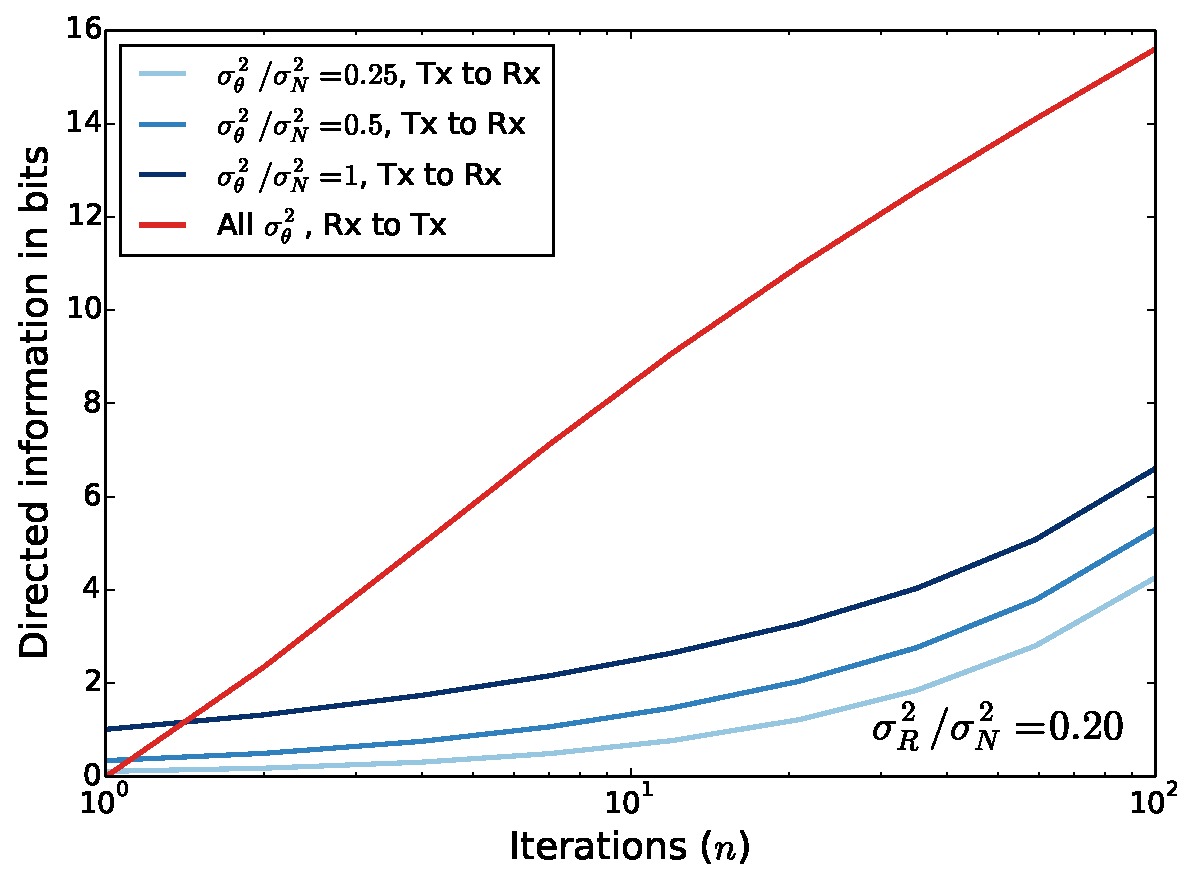
\includegraphics[width=3.2in]{noisy-fb-sigma_r2-point20} \\
	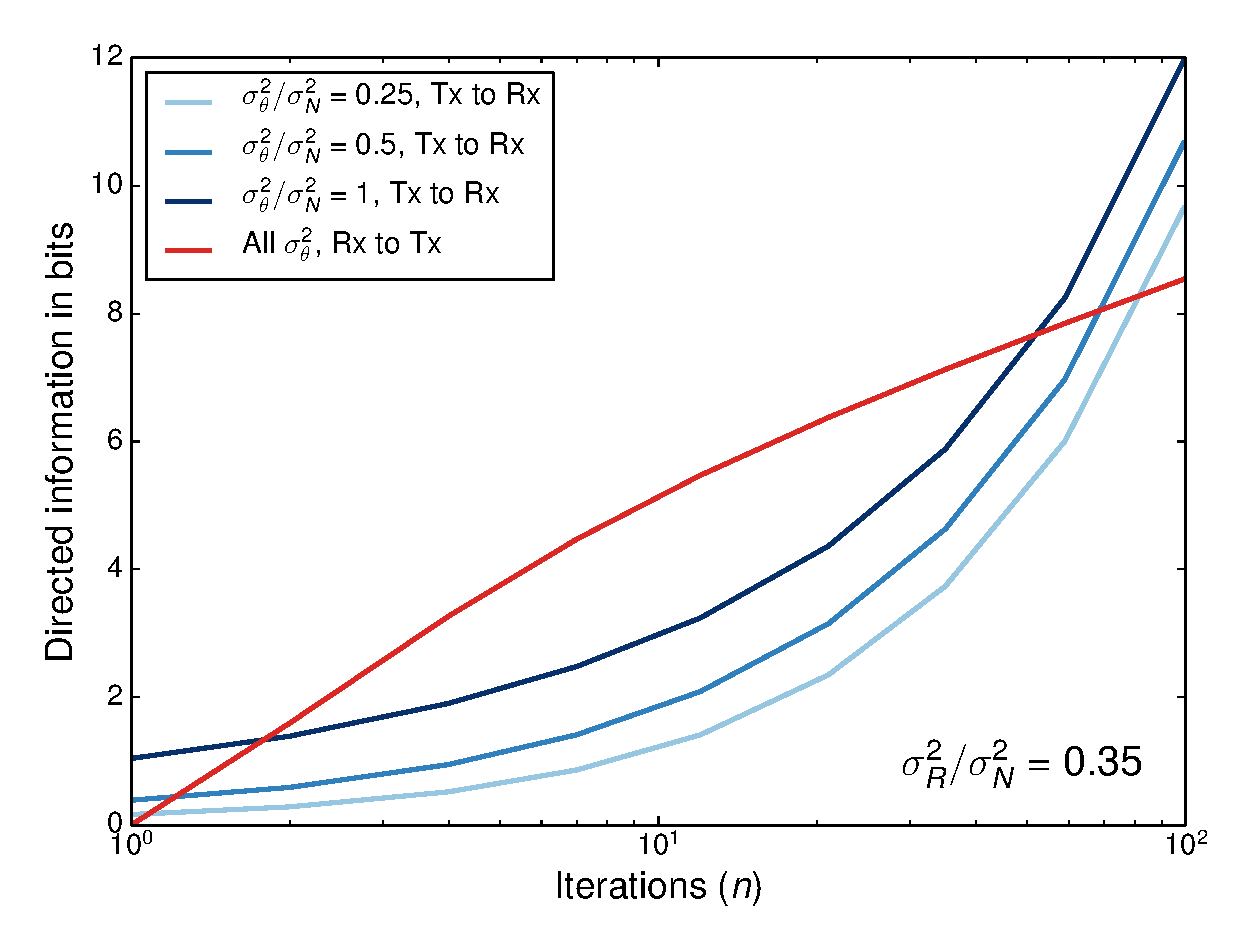
\includegraphics[width=3.2in]{noisy-fb-sigma_r2-point35} \\
	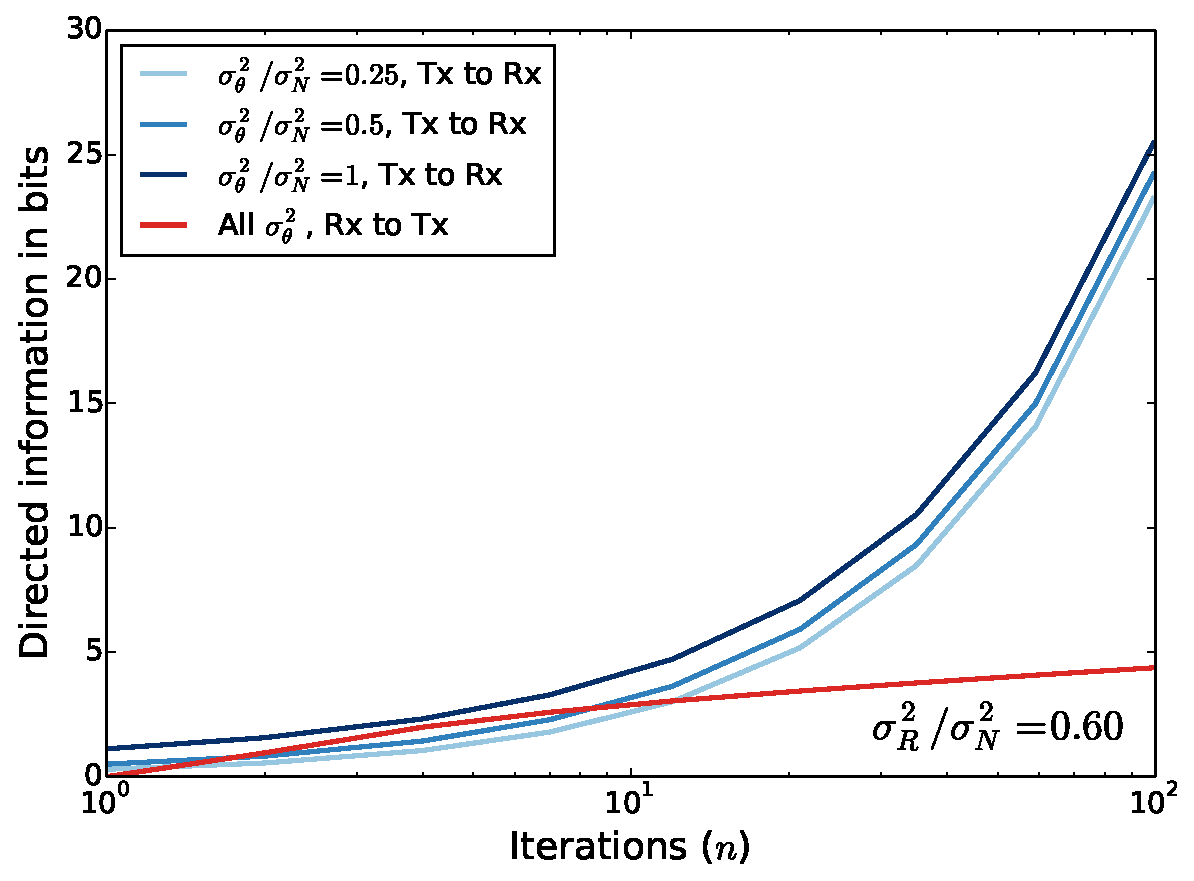
\includegraphics[width=3.2in]{noisy-fb-sigma_r2-point60}
	\caption{Plots for forward and backward directed information computations for ${\sigma_R^2}/{\sigma_N^2}=0.2$ (top), $0.35$ (center) and $0.6$ (bottom). In each plot, curves for directed information in both directions are illustrated for ratios ${\sigma_\theta^2}/{\sigma_N^2} = 0.25, 0.5,$ and $1$. The x-axis is the number of iterations of message-passing between the transmitter and the receiver. For cases when feedback noise variance $\sigma_R^2$ is moderately smaller than feedforward noise variance $\sigma_N^2$, directed information in the reverse link can dominate that in the forward link. With sufficiently many (albeit sometimes large, as illustrated in the top figure) iterations, directed information in forward information starts to dominate. However, the point at which this happens depends on the (often unknown) ratio of noise in these links. }
		     \label{fig:numerical}
\end{figure}

% Conclusions and discussions -------------------------------------------------

\section{Conclusions and discussions}
\label{sec:conclusions}

We demonstrate, by means of a concrete counter-example, that the direction predicted by causal influence metrics such as Granger Causality and Directed Information can be opposite to the true direction of information flow. There are, however, several shortcomings to our analysis, which we list in section~\ref{sec:objections-and-shortcomings}. We seek to address many of these shortcomings in future work.

It might appear that we make a circular argument while computing the Granger Causal influences in our counter-example, since we supply the model for the stochastic process and use the system parameters of the model directly to compute the Granger Causality metric. However, as we state in Section~\ref{sec:estimating-ar-coeffs}, we assume that the regression coefficients of the Autoregressive model can be exactly estimated (even if the AR process is non-stationary), and discuss how this might be achieved with the help of multiple trials.

As a final remark, we emphasize that this work only demonstrates the error in \emph{interpreting} the direction of causal influence as the direction of \emph{information flow}. We do \emph{not} seek to invalidate much of the neuroscientific work that has been done in this direction; we merely caution against making (what might be construed as hopeful) extrapolations from causal influences as to the manner in which information flows.

We do not seek to understate the importance of determining causal influences in the brain; understanding causal influence itself may have a great deal of benefit. For instance, we might seek to understand the spread of activity in the brain during an epileptic siezure -- in such applications, we are not concerned with how information is being transferred through the neural circuitry; we only seek to determine the source of the activity for the purpose of surgical intervention.

%We note that Granger's original analysis does not compare Granger causality on forward and reverse links. We are doing so, in part because it is often done in practice. It strikes us that this is being done because of the ``conservation of directed information'', an equality first derived by Massey~\cite{massey2005conservation}. This equality, which states that the sum of forward and reverse Directed Informations is the mutual information, could be viewed as suggesting that an increase in Directed Information in one direction must reduce it in the other direction. However, this is not true. For e.g., making $X$ and $Y$ uncorrelated reduces Directed Information in both directions (along with their sum) to zero. In other words, Massey's law is not a conservation law in the sense of conservation laws of energy, momentum, or mass, where the total energy/momentum/mass (\textit{i.e.}, the RHS) remains conserved (\textit{i.e.}, constant) regardless of the experiment performed on the entities.

% TODO: Include in final version:
% Some of this misconception might have arisen because of Massey's directed info conservation - we expect that dir info in the forward dirn goes up if the other one goes down - but this is a misnomer. (Do we still need this? I am increasingly of the opinion that directed info / GC capture nothing about the message)

% Acknowledgements ------------------------------------------------------------

\section*{Acknowledgments}

The authors would like to thank Nicola Elia for discussions that suggested this possible misunderstanding in use of Granger causality and Directed Information in computational systems. We also thank Rob Kass, Momin Malik and Kun Zhang for useful discussions. Finally, we thank the reviewers of a previous submission of this work to ISIT for their insightful remarks and comments. Praveen Venkatesh is partially supported by a dean's fellowship. %Pulkit Grover is supported by [...].

\bibliographystyle{IEEEtran}
\bibliography{IEEEabrv,references}

\newpage

\appendices

\section{Directed Information in the forward direction, noiseless feedback}
\label{app:dir-info-fwd-noiseless}

The Directed Information in the forward direction is computed as:
\begin{align*}
	I(X^n \rightarrow \widehat\Theta^n) &= \sum_{i=1}^n{I(\widehat\Theta_i ; X^i | \widehat\Theta^{i-1})} \\
										&= \sum_{i=1}^n{h(\widehat\Theta_i | \widehat\Theta^{i-1}) - h(\widehat\Theta_i | \widehat\Theta^{i-1}, X^i)} \numberthis \label{eq:dir-info-fwd-noiseless}
\end{align*}
Taking the first term in \eqref{eq:dir-info-fwd-noiseless},
\begin{align*}
	h(\widehat\Theta_i | \widehat\Theta^{i-1}) &= h \bigg( \widehat\Theta_{i-1} + \frac{X_i + N_i}{i} \bigg| \widehat\Theta^{i-1} \bigg) \\
											   &= h(\Theta - \widehat\Theta_{i-1} + N_i | \widehat\Theta^{i-1}) -\log(i) \\
											   &= h(\Theta + N_i | \widehat\Theta^{i-1}) -\log(i) \\
											   &= h(\Theta + N_i | \widehat\Theta_{i-1}) -\log(i)
\end{align*}
where we have dropped the conditioning on all except $\widehat\Theta_{i-1}$ in the last step. %TODO: Justify. Markov proof is too long to write here.
Define $U = \Theta + N_i$ and $V = \widehat\Theta_{i-1}$. Since all variables are Gaussian, it suffices to find the variance of the conditional distribution $U|V$.
\begin{align*}
	\mathbb{E}[U] = 0,
	\mathbb{E}[V] &= 0, \text{Var}[U] = \sigma_\theta^2 + \sigma_N^2,
	\text{Var}[V] = \sigma_\theta^2+ \frac{\sigma_N^2}{i-1} \\
	\text{Cov}[U,V] &= \mathbb{E}[UV]-\mathbb{E}[U]\mathbb{E}[V] \\
					&= \sigma_\theta^2 \\
	\rho^{2}        &= \frac{\sigma_{\theta}^{4}}{(\sigma_{\theta}^{2}+\sigma_{N}^{2})(\sigma_{\theta}^{2}+\frac{\sigma_{N}^{2}}{(i-1)})}
\end{align*}
\begin{equation*}
	U|V=v\ \sim\ \mathcal{N}\left(\sqrt{\frac{\sigma_{\theta}^{2}+\sigma_{N}^{2}}{\sigma_{\theta}^{2}+\frac{\sigma_{N}^{2}}{i-1}}}\rho v,(1-\rho^{2})(\sigma_{\theta}^{2}+\sigma_{N}^{2})\right)
\end{equation*}
Hence, the entropy of the conditional distribution is
\begin{equation*}
	h(U|V=v)=\frac{1}{2}\log(2\pi e(1-\rho^{2})(\sigma_{\theta}^{2}+\sigma_{N}^{2})) \overset{(a)}{=} h(U|V)
\end{equation*}
where (a) follows because the conditional entropy is independent of $v$. Thus,
\begin{equation}
	h(\widehat{\Theta}_{i}|\widehat{\Theta}^{i-1}) = \frac{1}{2}\log\left(2\pi e\frac{\sigma_{N}^{2}(i\sigma_{\theta}^{2}+\sigma_{N}^{2})}{((i-1)\sigma_{\theta}^{2}+\sigma_{N}^{2})}\right)-\log(i) \label{eq:htheta_theta-noiseless}
\end{equation}
The next term in equation \eqref{eq:dir-info-fwd-noiseless} is
\begin{align*}
	h(\widehat{\Theta}_{i}|\widehat{\Theta}^{i-1},X^{i}) &= h\left(\frac{N_{i}}{i}\bigg|\widehat{\Theta}^{i-1},X^{i}\right) \\
												 &= h(N_{i}) -\log(i) \\
												 &= \frac{1}{2}\log(2\pi e\sigma_{N}^{2}) -\log(i) \numberthis \label{eq:htheta_x_theta-noiseless}
\end{align*}
Putting equations \eqref{eq:htheta_theta-noiseless} and \eqref{eq:htheta_x_theta-noiseless} together, we can compute the forward Directed Information:
\begin{align*}
	I(\widehat{\Theta}_{i};X^{i}|\widehat{\Theta}^{i-1}) &= h(\widehat{\Theta}_{i}|\widehat{\Theta}^{i-1}) - h(\widehat{\Theta}_{i}|\widehat{\Theta}^{i-1},X^{i}) \\
	                                             &= \frac{1}{2}\log\left(\frac{i\sigma_{\theta}^{2}+\sigma_{N}^{2}}{(i-1)\sigma_{\theta}^{2}+\sigma_{N}^{2}}\right) \\
	I(X^{n} \rightarrow \widehat{\Theta}^{n})    &= \sum_{i=1}^{n}I(\widehat{\Theta}_{i};X^{i}|\widehat{\Theta}^{i-1}) \\
												 &\overset{(a)}{=} \frac{1}{2}\log\left(\frac{n\sigma_{\theta}^{2}+\sigma_{N}^{2}}{\sigma_{N}^{2}}\right) \\
	                                             &= \frac{1}{2}\log\left(1+\frac{n\sigma_{\theta}^{2}}{\sigma_{N}^{2}}\right)
\end{align*}
where (a) follows through by expanding out the product inside the logarithms and canceling terms. Clearly, this value is finite.

\section{Directed Information in the forward direction, with noisy feedback}
\label{app:dir-info-fwd-noisy}

\begin{align*}
	I(X^n \rightarrow \widehat\Theta^n) &= \sum_{i=1}^n{I(\widehat\Theta_i ; X^i | \widehat\Theta^{i-1})} \\
									 &= \sum_{i=1}^n{h(\widehat\Theta_i | \widehat\Theta^{i-1}) - h(\widehat\Theta_i | \widehat\Theta^{i-1}, X^i)}
\end{align*}
Taking the first of the two terms in the above expression,
\begin{align*}
	h(\widehat\Theta_i | \widehat\Theta^{i-1}) &\overset{(a)}{=} h(\widehat\Theta_{i-1} \frac{i-1}{i} + \frac{\Theta}{i} - \frac{R_{i-1}}{i} + \frac{N_i}{i} | \widehat\Theta^{i-1}) \\
											   &= h(\Theta - R_{i-1} + N_i | \widehat\Theta^{i-1}) -\log(i)
\end{align*}
where for (a) we have used equation \eqref{eq:theta_hat_i-noisy-once}. The Markov property no longer holds in this case, but we proceed in the same manner. We define $U = \Theta - R_{i-1} + N_i$ and $\underbar{V} = \widehat\Theta^{i-1}$. Recalling equation \eqref{eq:theta_hat_i-noisy}, for $j \in \{1, \ldots i-1\}$, $p \in \{1, \ldots i-1\}$ and $q \in \{1, \ldots i-1\}$, we have
\begin{align*}
	\mathbb{E}[U] &= 0,\;	\mathbb{E}[\widehat\Theta_j] = 0,\;\\	\mathbb{E}[U^2] &= \sigma_\theta^2 + \sigma_R^2 + \sigma_N^2,\;	\mathbb{E}[U \widehat\Theta_j] = \sigma_\theta^2 \\
	\mathbb{E}[\widehat\Theta_p \widehat\Theta_q] &= \mathbb{E} \bigg[ \bigg( \Theta + \frac{1}{p} \sum_{k=1}^p N_k - \frac{1}{p} \sum_{k=1}^{p-1} R_k \bigg)\\
												  & \qquad \qquad \bigg( \Theta + \frac{1}{q} \sum_{k=1}^q N_k - \frac{1}{q} \sum_{k=1}^{q-1} R_k \bigg) \bigg] \\
												  &= \sigma_\theta^2 + \frac{\min\{p, q\}}{pq} \sigma_N^2 + \frac{\min\{p-1, q-1\}}{pq} \sigma_R^2 \\
	\text{Var}[U|\widehat\Theta^{i-1}] &= \mathbb{E}[U^2] - \mathbb{E}[U \underbar{V}] \mathbb{E}[\underbar{V} \underbar{V}^T]^{-1} \mathbb{E}[\underbar{V} U] \\
	h(U | \widehat\Theta^{i-1}) &= \frac{1}{2}\log(2 \pi e \text{Var}[U | \widehat\Theta^{i-1}]) \numberthis \label{eq:h_theta_theta-noisy}
\end{align*}
We can not derive a simple closed form for this expression, but we have computed it numerically for the plots in Section~\ref{sec:numerical-results}. The second term in equation \eqref{eq:dir-info-fwd-noisy} is
\begin{align*}
	h(\widehat\Theta_i | \widehat\Theta^{i-1}, X^i) &= h \bigg( \widehat\Theta_{i-1} + \frac{X_i + N_i}{i} \bigg| \widehat\Theta^{i-1}, X^i \bigg) \\
													&= h(N_i | \widehat\Theta^{i-1}, X^i) -\log(i) \\
													&= \frac{1}{2}\log(2 \pi e \sigma_N^2) -\log(i) \numberthis \label{eq:h_theta_x_theta-noisy}
\end{align*}
From equations \eqref{eq:h_theta_theta-noisy} and \eqref{eq:h_theta_x_theta-noisy}, we compute the forward-directed information as depicted in Section~\ref{sec:numerical-results}, for different values of $\sigma_\theta^2$.

\section{Directed Information in the reverse direction, with noisy feedback}
\label{app:dir-info-rev-noisy}

\begin{align*}
	I(0*\widehat\Theta^{n-1} \rightarrow X^n) &= \sum_{i=0}^{n-1}{I(X_{i+1}; \widehat\Theta^i | X^i)} \\
											  &= \sum_{i=0}^{n-1}{h(X_{i+1} | X^i) - h(X_{i+1} | X^i, \widehat\Theta^i)} \numberthis
\end{align*}
Taking the first term inside the summation,
\begin{align*}
	h(X_{i+1} | X^i) &= h(\Theta - \widehat\Theta_i - R_i | X^i) \\
					&\overset{(a)}{=} h \bigg( \bigg( - \widehat\Theta_{i-1} - \frac{X_i + N_i}{i} \bigg) - R_i \bigg| X^i \bigg) \\
					&\overset{(b)}{=} h \bigg( \bigg( X_i - \Theta + R_{i-1} - \frac{N_i}{i} \bigg) - R_i \bigg| X^i \bigg) \\
					&\overset{(c)}{=} h \bigg( R_{i-1} - \frac{N_i}{i} - R_i \bigg| X^i \bigg)
\end{align*}
where in (a) above, we have dropped $\Theta = X_1$, in (b) we have re-expressed $\widehat\Theta_{i-1}$ in terms of $X_i$, $\Theta$ and $R_{i-1}$, and in (c) we have dropped $X_i$ and $\Theta$ again. As before, define $U = R_{i-1} - \frac{N_i}{i} - R_i$, so that
\begin{equation*}
	\mathbb{E}[U] = 0,\; \; \mathbb{E}[X_j] = 0, \; \; \mathbb{E}[U^2] = 2 \sigma_R^2 + \frac{\sigma_N^2}{i^2}
\end{equation*}
For $i \geq 3$ and $j \in \{3, \ldots i\}$, we can use equation \eqref{eq:x_i-noisy} to see that
\begin{align*}
	\mathbb{E}[U X_j] &= \mathbb{E} \bigg[ \bigg( R_{i-1} - \frac{N_i}{i} - R_i \bigg) \\
					  & \qquad             \bigg( \frac{1}{j-1} \sum_{k=1}^{j-2} R_k - \frac{1}{j-1} \sum_{k=1}^{j-1} N_k - R_{j-1} \bigg) \bigg] \\
					  &= - \mathbb{E}[R_{i-1} R_{j-1}] = - \sigma_R^2 \delta_{ij} \\
	\mathbb{E}[U X_1] &= \mathbb{E} \bigg[ \bigg( R_{i-1} - \frac{N_i}{i} - R_i \bigg) \Theta \bigg] = 0 \; \\
	\mathbb{E}[U X_2] &= \mathbb{E} \bigg[ \bigg( R_{i-1} - \frac{N_i}{i} - R_i \bigg) (\Theta - (\Theta + N_i) - R_1) \bigg] = 0 \; \\
	\mathbb{E}[X_p X_q] &= \mathbb{E} \bigg[ \bigg( \frac{1}{p-1} \sum_{k=1}^{p-2} R_k - \frac{1}{p-1} \sum_{k=1}^{p-1} N_k - R_{p-1} \bigg) \\
						& \qquad             \bigg( \frac{1}{q-1} \sum_{k=1}^{q-2} R_k - \frac{1}{q-1} \sum_{k=1}^{q-1} N_k - R_{q-1} \bigg) \bigg] \\
					    &= \frac{\min\{p-2, q-2\}}{(p-1)(q-1)} \sigma_R^2 + \frac{\min\{p-1, q-1\}}{(p-1)(q-1)} \sigma_N^2 \\
						& \qquad + \sigma_R^2 \delta_{pq} + \frac{1}{p-1} \sigma_R^2 \mathbb{I}_{p>q} + \frac{1}{q-1} \sigma_R^2 \mathbb{I}_{q>p} \\
	\mathbb{E}[X_1 X_1] &= \mathbb{E}[\Theta^2] = \sigma_\theta^2 \\
	\mathbb{E}[X_1 X_j] &= \mathbb{E} \bigg[ \Theta \bigg( \frac{1}{j-1} \sum_{k=1}^{j-2} R_k - \frac{1}{j-1} \sum_{k=1}^{j-1} N_k - R_{j-1} \bigg) \bigg] = 0 \\
	\text{Var}[U|X^i] &= \mathbb{E}[U^2] - \mathbb{E}[U X^i] \mathbb{E}[X^i {X^i}^T]^{-1} \mathbb{E}[X^i U] \\
	h(U | X^i) &= \frac{1}{2}\log(2 \pi e \text{Var}[U | X^i]) \numberthis \label{eq:h_x_x-noisy}
\end{align*}
The above argument can be extended to $i=2$ by letting the final index of the summation term be smaller than the starting index, implying that the whole summation term is simply dropped. The special cases of $i=0$ and $i=1$ are handled at the end. The second term from equation \eqref{eq:dir-info-rev-noisy} becomes
\begin{align*}
	h(X_{i+1} | X^i, \widehat\Theta^i) &= h(\Theta - \widehat\Theta_i - R_i | X^i, \widehat\Theta^i) \\
									   &= \frac{1}{2}\log(2 \pi e \sigma_R^2) \numberthis \label{eq:h_x_x_theta-noisy}
\end{align*}
because $X_1 = \Theta$ and because $R_i$ is independent of all the $X^i$ and $\widehat\Theta^i$. For the special cases of $i=0$ and $i=1$, we solve for the value of mutual information explicitly:
\begin{align*}
	i = 0: & \qquad I(X_1; \widehat\Theta^0 | X^0) &=& \; h(X_1) - h(X_1) = 0 \\
	i = 1: & \qquad I(X_2; \widehat\Theta^1 | X^1) &=& \; h(X_2 | X_1) - h(X_2 | X_1, \widehat\Theta_1) \\
		   & \qquad h(X_2 | X_1)                   &=& \; h(\Theta - \widehat\Theta_1 - R_1 | X^1) \\
		   & \qquad                                &=& \; h(-\Theta - N_1 - R_1 | X_1) \\
		   & \qquad                                &=& \; h(-N_1 - R_1) \\
		   & \qquad                                &=& \; \frac{1}{2} \log(2 \pi e (\sigma_N^2 + \sigma_R^2)) \\
		   & \qquad h(X_2 | X_1, \widehat\Theta_1) &=& \; h(-R_1) = \frac{1}{2} \log(2 \pi e \sigma_R^2) \\
		   & \qquad I(X_2; \widehat\Theta^1 | X^1) &=& \; \frac{1}{2} \log \bigg( 2 \pi e \frac{\sigma_N^2 + \sigma_R^2}{\sigma_R^2} \bigg)
\end{align*}
From equations \eqref{eq:h_x_x-noisy} and \eqref{eq:h_x_x_theta-noisy}, along with the two special cases above, we can now compute the reverse-directed information plotted in Section~\ref{sec:numerical-results}.




% trigger a \newpage just before the given reference
% number - used to balance the columns on the last page
% adjust value as needed - may need to be readjusted if
% the document is modified later
%\IEEEtriggeratref{14}
% The "triggered" command can be changed if desired:
%\IEEEtriggercmd{\enlargethispage{-5in}}

% references section

% can use a bibliography generated by BibTeX as a .bbl file
% BibTeX documentation can be easily obtained at:
% http://www.ctan.org/tex-archive/biblio/bibtex/contrib/doc/
% The IEEEtran BibTeX style support page is at:
% http://www.michaelshell.org/tex/ieeetran/bibtex/
%\bibliographystyle{IEEEtran}
% argument is your BibTeX string definitions and bibliography database(s)
%\bibliography{IEEEabrv,../bib/paper}
%
% <OR> manually copy in the resultant .bbl file
% set second argument of \begin to the number of references
% (used to reserve space for the reference number labels box)




% that's all folks
\end{document}


